%% 
%% Copyright 2007, 2008, 2009 Elsevier Ltd
%% 
%% This file is part of the 'Elsarticle Bundle'.
%% ---------------------------------------------
%% 
%% It may be distributed under the conditions of the LaTeX Project Public
%% License, either version 1.2 of this license or (at your option) any
%% later version.  The latest version of this license is in
%%    http://www.latex-project.org/lppl.txt
%% and version 1.2 or later is part of all distributions of LaTeX
%% version 1999/12/01 or later.
%% 
%% The list of all files belonging to the 'Elsarticle Bundle' is
%% given in the file `manifest.txt'.
%% 

%% Template article for Elsevier's document class `elsarticle'
%% with numbered style bibliographic references
%% SP 2008/03/01

\documentclass[preprint,12pt, a4paper]{elsarticle}

%% Use the option review to obtain double line spacing
%% \documentclass[authoryear,preprint,review,12pt]{elsarticle}

%% For including figures, graphicx.sty has been loaded in
%% elsarticle.cls. If you prefer to use the old commands
%% please give \usepackage{epsfig}

%% The amssymb package provides various useful mathematical symbols
\usepackage{amssymb}
\usepackage{hyperref}
\usepackage{float}
\setlength{\parindent}{0pt}
\usepackage{listings}
\usepackage{xcolor}
\usepackage{amsmath}
\usepackage{amssymb}
\usepackage{tabularx}
\usepackage{array}
\usepackage{booktabs}
\usepackage{array}
\usepackage{tabularx}
\usepackage{xltabular}
\usepackage{ltablex}
\usepackage{booktabs}
\usepackage{xltabular}
\usepackage{array}
\usepackage{ragged2e}
\usepackage{url}
\usepackage{xcolor}
\usepackage{graphicx}
\keepXColumns
% Define Python style for listings
\lstdefinestyle{pythonStyle}{
    language=Python,
    backgroundcolor=\color{gray!10},
    basicstyle=\ttfamily\footnotesize,
    keywordstyle=\color{blue}\bfseries,
    stringstyle=\color{orange},
    commentstyle=\color{green!60!black}\itshape,
    showstringspaces=false,
    numbers=left,
    numberstyle=\tiny\color{gray},
    frame=single,
    breaklines=true,
    postbreak=\mbox{\textcolor{red}{$\hookrightarrow$}\space}
}
%% The amsthm package provides extended theorem environments
%% \usepackage{amsthm}

%% The lineno packages adds line numbers. Start line numbering with
%% \begin{linenumbers}, end it with \end{linenumbers}. Or switch it on
%% for the whole article with \linenumbers.
%\usepackage{lineno}

\journal{SoftwareX}

\begin{document}
\renewcommand{\labelenumii}{\arabic{enumi}.\arabic{enumii}}

\begin{frontmatter}

\title{MobileSec: A Microservices-Based Intelligent Platform for Automated Android APK Vulnerability Analysis and Remediation.}

%% use optional labels to link authors explicitly to addresses:
%% \author[label1,label2]{}
%% \address[label1]{}
%% \address[label2]{}

\author[label1]{Abdelali Ayoujil}
\author[label1,label2]{Mohamed Lachgar}
\author[label3]{Omar Achbarou}
\author[label4]{Mohamedou Cheikh Tourad}

\address[label1]{Cadi Ayyad University, I2IS Laboratory, Marrakech, Morocco}
\address[label2]{Cadi Ayyad University, Higher Normal School (ENS), Computer Science Department, Marrakech, Morocco}
\address[label3]{Cadi Ayyad University, National School of Applied Sciences, IMSC Laboratory, Marrakech, Morocco}
\address[label4]{University of Nouakchott, Faculty of Sciences and Techniques, Al-Khawarizmi,  Nouakchott, Mauritania}

\begin{abstract}
\textit{MobileSec} is an open-source platform for the static security analysis of Android application packages (APKs), designed around a modular microservices architecture. The platform automates security assessment by combining APK preprocessing with specialized analysis services that detect issues such as cryptographic misuse, hard-coded secrets, and insecure network configurations. To help users focus on the most important findings, MobileSec incorporates a LightGBM-based model for vulnerability prioritization, producing ranked results with confidence estimates. The platform also includes an AI-assisted remediation component that provides vulnerability explanations, mitigation guidance, and Java/Kotlin-oriented fix suggestions through large language model integration. Its containerized design \textcolor{blue}{supports reproducible containerised deployment and benchmark-based experimentation}, making the platform useful for researchers, security analysts, and developers working on Android application security. \textcolor{blue}{MobileSec also integrates a LightGBM-based prioritisation module that converts
heterogeneous scan findings into ranked remediation categories.}
\end{abstract}

\begin{keyword}
Android security; APK static analysis; machine learning; AI-assisted remediation
\end{keyword}

\end{frontmatter}

%\linenumbers

\section*{Metadata}
\begin{table}[H]
\caption{Code metadata}
\label{codeMetadata}
\centering
\footnotesize
\renewcommand{\arraystretch}{1.15}
\begin{tabular}{p{0.12\linewidth} p{0.38\linewidth} p{0.45\linewidth}}
\hline
\textbf{Nr} & \textbf{Code metadata description} & \textbf{Metadata} \\
\hline

C1 & Current code version 
& v1.0.0 \\

C2 & Permanent link to code/repository used for this code version 
& \url{https://github.com/ayoujil200/mobilesec} \\

C3 & Permanent link to reproducible capsule 
& \url{https://github.com/ayoujil200/mobilesec} \\

C4 & Legal code license 
& MIT License \\

C5 & Code versioning system used 
& Git \\

C6 & Software code languages, tools, and services used 
& Python, Kotlin, JavaScript, Docker \\

C7 & Compilation requirements, operating environments and dependencies 
& Docker Engine, Python 3.10+, Node.js 18+, Androguard, LightGBM, Flask, Spring Boot, React \\

C8 & If available, link to developer documentation/manual 
& \textcolor{blue}{\url{https://github.com/ayoujil200/mobilesec/blob/dev/docs/developer-guide.md}} \\

C9 & Support email for questions 
& \texttt{a.ayoujil.ced@uca.ac.ma} \\

\hline
\end{tabular}
\end{table}

\section{Motivation and significance}

%% humanized
Android applications make up a major portion of the mobile software ecosystem and, as a result, are common targets for security threats such as malware injection, credential leakage, improper use of cryptographic mechanisms, and insecure network communication \cite{arzt2014flowdroid, enck2014taintdroid}. Static analysis has long served as a scalable method for identifying these vulnerabilities, but many existing Android security analysis tools remain limited in scope. They often concentrate on specific vulnerability types, depend heavily on rule-based detection methods, or generate large numbers of findings without clear prioritization \cite{feng2014apposcopy, li2017iccta}. In addition, many tools do not provide built-in support for interpreting vulnerabilities or guiding remediation, which forces analysts to manually connect results across different and often inconsistent toolchains. Together, these shortcomings reduce scalability, reproducibility, and efficiency in both research-oriented and industry-based Android security assessments.

%% humanized
The development of \textit{MobileSec} is motivated by the need for an integrated and extensible software platform that consolidates static APK analysis, vulnerability prioritization, and remediation support within a unified framework. The software is designed to address the scientific problem of transforming low-level static analysis outputs into actionable, ranked security insights. By combining multiple analysis techniques into a modular pipeline, MobileSec reduces fragmentation in Android security workflows and enables systematic experimentation with vulnerability detection and ranking strategies, building on foundations provided by widely used tools such as Androguard \cite{desnos2011androguard} and benchmark suites like DroidBench \cite{arzt2014droidbench}.

%% humanized
MobileSec contributes to the process of scientific discovery in mobile security research by supporting reproducible and extensible experimentation. Its microservices-based architecture allows individual analysis components---including cryptographic misuse detection, secret leakage analysis, and network security inspection---to be independently developed, evaluated, and replaced. This design facilitates comparative studies of static analysis techniques and enables the integration of machine learning--based methods for vulnerability assessment \cite{liu2021mlsecurity}. In particular, the inclusion of a LightGBM-based classifier \cite{ke2017lightgbm} enables data-driven prioritization of detected vulnerabilities, allowing researchers to study the impact of different feature representations and ranking models on vulnerability triage effectiveness.

%% not humanized
\textcolor{blue}{In addition to detecting vulnerabilities, MobileSec addresses the practical
problem of deciding which remediation action should be handled first. Static
analysis services can produce many heterogeneous findings for the same APK,
including cryptographic misuse, exposed credentials, insecure HTTP endpoints,
and TLS validation weaknesses. MobileSec therefore adds a prioritisation layer
that summarises scan-level evidence and predicts the most relevant remediation
category for the analysed application.}

%% humanized
From both an experimental and user-oriented perspective, MobileSec serves as a fully integrated end-to-end static analysis pipeline. Users submit Android APK files through a web-based interface, after which the platform automatically performs static analysis using specialized services. The resulting findings are then aggregated, scored, and presented through interactive dashboards and structured reports that can be exported for deeper examination. In addition, an optional AI-assisted remediation module provides explanatory insights and code-level fix suggestions, allowing researchers to evaluate automated vulnerability explanation and mitigation support enabled by large language models. \cite{pearce2022copilot,white2023prompt}

%% humanized
MobileSec expands on and works alongside existing Android security analysis tools and frameworks, including decompilation-based analyzers, rule-based static scanners, and approaches that follow industry standards such as the OWASP Mobile Application Security Verification Standard (MASVS) \cite{owaspmasvs}. While many current solutions concentrate mainly on identifying vulnerabilities, MobileSec gives greater attention to modular deployment, automated vulnerability prioritization, and built-in remediation support. Together, these features make the software valuable both as a practical research platform for Android security analysis and as a tool that can be applied in real-world security assessment workflows.

\section{Software description}

%% humanized
\textit{MobileSec} is a containerized platform built on a microservices architecture for assessing the security of Android applications. It is designed to analyze uploaded APK and AAB files, store both intermediate and final analysis results in MongoDB, and provide outputs that are suitable for both machine processing and human interpretation in research and operational settings. The current implementation integrates deterministic static analysis checks, service-level orchestration, model-driven vulnerability prioritization, and AI-assisted remediation guidance.

%% humanized
In practice, MobileSec structures its analysis workflow as a staged pipeline that includes artifact ingestion, APK preprocessing, specialized security analysis, vulnerability aggregation, prioritization, remediation recommendation, and report export. This design allows each security module, such as crypto, secrets, network, ML, and reporting, to evolve independently without the need for a monolithic redesign.

\subsection{Software architecture}

The figure~\ref{fig:arch} gives an overview of the MobileSec architecture, highlighting how its main services work together and how data flows through the analysis process.

\begin{figure}[htbp]
    \centering
    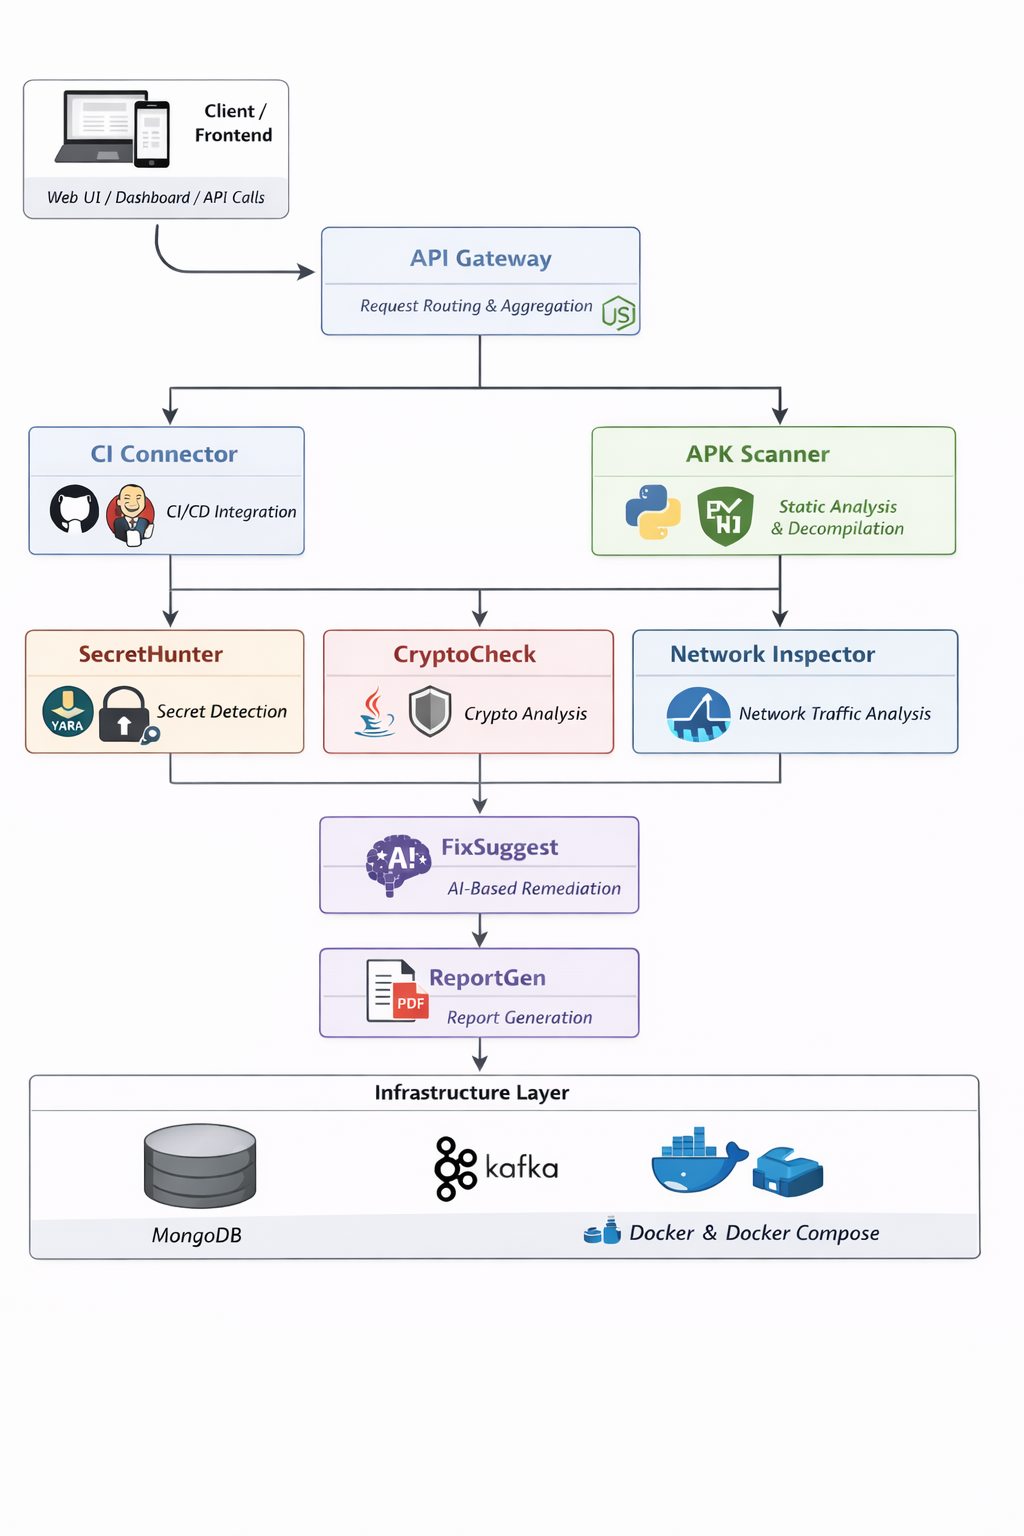
\includegraphics[width=\linewidth]{figures/Archi.png}
    \caption{\textcolor{blue}{Overview of the MobileSec architecture illustrating service interaction and data flow.}}
    \label{fig:arch}
\end{figure}

\textcolor{blue}{MobileSec adopts a modular microservices architecture in which each major stage of the analysis pipeline is implemented as a separate service. This organization separates analysis responsibilities and supports independent evolution of detectors and reporting components. Communication between services combines synchronous REST-based requests with asynchronous event-driven messaging. The architecture can support concurrent dispatch, but the stable quantitative evaluation reported in this article uses sequential APK execution.}

User interaction takes place through a web-based Frontend Dashboard that allows users to submit APKs, monitor scan progress in real time, and view structured analysis results. The dashboard communicates only with the API Gateway, which preserves the abstraction of the underlying internal architecture.

The architecture is organized around the following main services:

\begin{itemize}
    \item \textbf{API Gateway}: At the system’s entry point, an API Gateway serves as the central interface between the frontend dashboard and the backend services. It is responsible for validating incoming requests, handling APK uploads, routing traffic to the appropriate analysis components, and exposing structured API documentation. By separating client interactions from the internal services, the gateway improves maintainability and helps enforce controlled access to system resources.

    \item \textbf{APK Scanner}: The main static analysis process begins in the APK Scanner service. This component automatically disassembles submitted APK files and extracts relevant artifacts, such as bytecode representations, manifest declarations, permissions, exported components, and embedded resources. It also detects network endpoints and configuration settings. After preprocessing is completed, the scanner emits structured events to the message broker, which then triggers the specialized analysis services.

    \item \textbf{SecretHunter}: The SecretHunter service is responsible for detecting hardcoded credentials and other sensitive information. It examines decompiled source artifacts using pattern-based and rule-driven techniques to uncover API keys, authentication tokens, private keys, and other embedded secrets. The service produces structured findings that are supplemented with relevant contextual metadata.

    \item \textbf{CryptoCheck}: Cryptographic implementations are analyzed by the CryptoCheck service. This component reviews code structures to identify insecure algorithm choices, weak hash functions, poor key management practices, hardcoded salts, and unsafe initialization vectors. By concentrating specifically on cryptographic correctness, it delivers focused analysis in one of the most security-sensitive areas of mobile application security.

    \item \textbf{Network Inspector}: Security issues related to networking are evaluated by the Network Inspector. This service reviews extracted endpoints and communication settings to identify insecure transport protocols, missing certificate validation, improper certificate pinning, and possible communication with untrusted domains.

    \item \textbf{Machine Learning Model}: In addition to rule-based analysis, MobileSec includes a dedicated Machine Learning Model service. This component classifies applications and vulnerability patterns using trained models to detect suspicious behavior or malware-related characteristics that may be missed by deterministic static rules. By relying on patterns learned from labeled datasets, the model helps broaden overall detection coverage.

    \item \textbf{FixSuggest}: To support remediation, the FixSuggest service produces structured explanations and recommended fixes for identified vulnerabilities. It combines predefined remediation templates with large language model (LLM)-based generation to create contextualized, code-level guidance, helping reduce the effort required to understand and address security issues.

    \item \textbf{MongoDB}: All findings generated by the analysis services are aggregated and stored in a centralized MongoDB database. This persistent storage supports traceability of scan results, reproducibility of experiments, and historical comparison across different application versions.

    \item \textbf{Report Generation (ReportGen)}: A dedicated Report Generation (ReportGen) service compiles vulnerability findings into structured outputs, including machine-readable summaries and stakeholder-focused documents such as PDF and HTML reports. In this way, the service converts raw analysis results into more understandable and actionable security assessments.

    \item \textbf{CI Connector}: To support automated DevSecOps practices, a CI Connector service allows the platform to integrate with continuous integration and deployment pipelines. As a result, security scans can be triggered automatically during build processes, embedding security assessment directly into the software development lifecycle.

    \item \textbf{Apache Kafka and Docker}: \textcolor{blue}{Communication between services is supported by Apache Kafka, which serves as the platform's messaging backbone. Kafka enables asynchronous and decoupled delivery of scan events to specialized services. The entire platform is containerized with Docker, which helps ensure reproducible deployments and consistent runtime environments across development and evaluation settings.}
\end{itemize}

The overall process, beginning with APK submission and continuing through distributed analysis, intelligent classification, remediation support, and report generation, is illustrated in Fig.~\ref{fig:arch}. MobileSec’s modular design also supports extensibility, making it possible to add new security services without affecting the existing components.

{\color{blue}\paragraph{Architectural trade-offs and failure management.}
The separation of scanning, specialized detection, prioritisation and reporting services improves modularity and makes individual components easier to extend. It also introduces communication, deployment, monitoring and recovery overhead that would be smaller in a single-process analyzer.

Kafka-based messaging and REST notifications require explicit treatment of service unavailability and partial results. In the implemented workflow, the scanner retries downstream notifications, preserves a partial or unavailable status when a downstream service cannot provide a result, and exposes a manual replay mechanism. A durable dead-letter queue is not part of the current implementation.

During evaluation, exploratory execution with four APK scans in parallel produced incomplete analyzer outcomes through time-outs or HTTP 404 responses. Consequently, the final 283-APK benchmark was executed with one APK scan at a time. The present study therefore does not claim a verified parallel throughput advantage, and it does not include a measured monolithic baseline.}

\subsection{Machine Learning-Based Vulnerability Prioritization}

{\color{blue}MobileSec uses a LightGBM multiclass classifier to prioritise remediation after static analysis. The model consumes 24 scan-level attributes produced by the cryptographic, secret-detection and network-analysis services, including finding counts, severity distributions, vulnerability-type indicators and an aggregate severity score. Its output is an operational remediation category, such as weak-cipher replacement, exposed-secret removal, HTTPS enforcement or certificate-validation repair. These categories support triage within the platform and can be mapped to relevant OWASP MASVS areas where appropriate; they are not presented as official OWASP labels or as direct estimates of exploitation risk.

The classification experiment uses labelled remediation outcomes retained by the MobileSec extraction pipeline together with their provenance metadata. Stratified training, validation and test partitions are used, and the selected LightGBM configuration optimises validation macro-F1 to account for class-wise performance.}

{\color{blue}
\begin{table}[H]
\centering
\caption{Configuration of the LightGBM remediation-prioritisation model.}
\label{tab:lightgbm-configuration}
\begin{tabular}{ll}
\toprule
\textbf{Parameter} & \textbf{Value} \\
\midrule
Input attributes & 24 scan-level attributes \\
Objective / metric & multiclass / multi\_logloss \\
Number of output classes & 12 \\
Boosting type & gbdt \\
Number of leaves & 7 \\
Learning rate & 0.08 \\
Bagging fraction / frequency & 0.8 / 5 \\
Minimum child samples & 4 \\
Regularisation $(\alpha,\lambda)$ & $(0.3, 0.6)$ \\
Maximum boosting rounds & 3000 \\
Early-stopping rounds & 150 \\
Random seed & 42 \\
\bottomrule
\end{tabular}
\end{table}
}

\subsection{Software functionalities}

MobileSec currently provides the following implemented capabilities:

\begin{enumerate}
    %% humanized
    \item \textbf{APK ingestion and scan lifecycle management:} Handling APK uploads and managing the scan lifecycle, including scan ID generation, stage-level status tracking, and monitoring the health of individual services.

    %% humanized
    \item \textbf{APK structural and manifest analysis:} Extraction of package metadata, permissions, exported components, debuggable and cleartext settings, certificate details, DEX statistics, and potential endpoint candidates.

    %% humanized
    \item \textbf{Multi-domain vulnerability detection:} Specialized security findings derived from cryptographic analysis, secret leakage detection, and network security inspection.

    %% humanized
    \item \textbf{Asynchronous orchestration:} Coordinated fan-out execution across services through REST-based notifications and Kafka topic consumption, with scan-state data persisted in MongoDB to support reproducibility.

    %% humanized
    \item \textbf{Data-driven prioritization:} LightGBM-based prediction of remediation categories, along with confidence-ranked recommendations generated from engineered features collected across multiple services.
    
    \item \textbf{AI-assisted remediation:} MASVS-guided and LLM-enhanced vulnerability explanations, prioritized remediation guidance, and patch suggestions tailored for Java and Kotlin.
    
    \item \textbf{Report generation and export:} Findings are consolidated, cleaned, and scored before being presented in the dashboard and exported in PDF, JSON, and SARIF formats.
    
    \item \textbf{DevSecOps integration support:} generation of CI templates and trigger endpoints to embed security scanning into automated build pipelines.
\end{enumerate}

\subsection{Sample code snippets analysis}

The function \texttt{perform\_complete\_scan} illustrates a complete static analysis pipeline for an Android APK. 
It orchestrates multiple stages, including structural bytecode analysis, manifest parsing using \texttt{ManifestParser}, 
permission-based risk assessment with \texttt{PermissionsAnalyzer}, and extraction of sensitive data such as API keys and network endpoints. 
The results are consolidated into a comprehensive security score and stored for further processing or notification to downstream services. 
This snippet highlights the integration of various tools and analyses into a single automated workflow for Android security evaluation.

\begin{lstlisting}[style=pythonStyle]
def perform_complete_scan(scan_id, apk_path):
    """
    Orchestrates the multi-stage static analysis pipeline for an Android APK.
    Combines manifest parsing, bytecode analysis, and risk scoring.
    """
    results = {
        'scan_id': scan_id,
        'timestamp': datetime.utcnow().isoformat(),
        'status': 'in_progress'
    }

    try:
        # 1. Structural Analysis (Bytecode/Resources)
        # Uses Androguard to extract basic metadata and compiled strings
        androguard = AndroguardWrapper(apk_path)
        androguard.load_apk()
        basic_info = androguard.get_basic_info()

        # 2. Manifest & Decompilation (External Tool Integration)
        # Invokes Apktool to reconstruct original XML configurations
        manifest_parser = ManifestParser(apk_path)
        decompiled_path = os.path.join(DECOMPILED_FOLDER, scan_id)
        manifest_parser.decompile_apk(decompiled_path)
        manifest_data = manifest_parser.parse_manifest()

        # 3. Behavioral Risk Assessment (Permissions)
        # Evaluates the permission model and calculates a weighted risk score
        analyzer = PermissionsAnalyzer()
        perm_analysis = analyzer.analyze_permissions(basic_info.get('permissions', []))

        # 4. Static Data Extraction (Secrets & Endpoints)
        # Performs regex-based pattern matching on Dalvik strings
        results.update({
            'package_name': basic_info['package_name'],
            'debuggable': manifest_data.get('debuggable', False),
            'permissions_risk': perm_analysis['risk_score'],
            'endpoints': androguard.extract_network_endpoints(),
            'secrets': androguard.get_api_keys(),
            'certificate': androguard.get_certificate_info()
        })

        # 5. Global Security Scoring
        # Synthesizes all findings into a normalized security metric (0-100)
        results['security_score'] = calculate_security_score(results)
        results['status'] = 'completed'

        # Persistent Storage & Inter-service Communication
        mongodb_client.save_scan_results(scan_id, results)
        produce_scan_event(scan_id, apk_path) # Notify downstream microservices (Kafka)

        return results

    except Exception as e:
        logger.error(f"Orchestration failure: {e}")
        return {'scan_id': scan_id, 'status': 'failed', 'error': str(e)}
\end{lstlisting}

\section{Illustrative examples}

This section presents representative usage scenarios demonstrating how MobileSec is used in practice to perform Android application security analysis, vulnerability prioritization, and remediation support.

\subsection{End-to-end static analysis of an Android APK}

%% humanized
In a typical workflow, a developer or security analyst uploads an Android application package (APK) through the web-based interface. The frontend includes a drag-and-drop upload feature and shows scan progress in real time. After submission, the CI-Connector service manages the analysis pipeline by routing the APK to the appropriate scanning services.

%% humanized
\textcolor{blue}{The APK-Scanner service decompiles the application and extracts key resources, bytecode and configuration files. It then dispatches the extracted evidence to specialized services: CryptoCheck identifies cryptographic misuse, SecretHunter searches for hard-coded secrets, and NetworkInspector reviews network configurations for insecure communication patterns and TLS-related weaknesses.}

%% humanized
The scan results are then consolidated and displayed on the main dashboard, which provides an overview of detected vulnerabilities by category, severity level, and scan status (Fig.~\ref{fig:dashboard}). Users can explore each category in more detail to review specific findings, including file paths, line references, and vulnerability descriptions. Overall, this workflow allows a full static security assessment of an APK to be carried out within a single platform.

\begin{figure}[H]
    \centering
    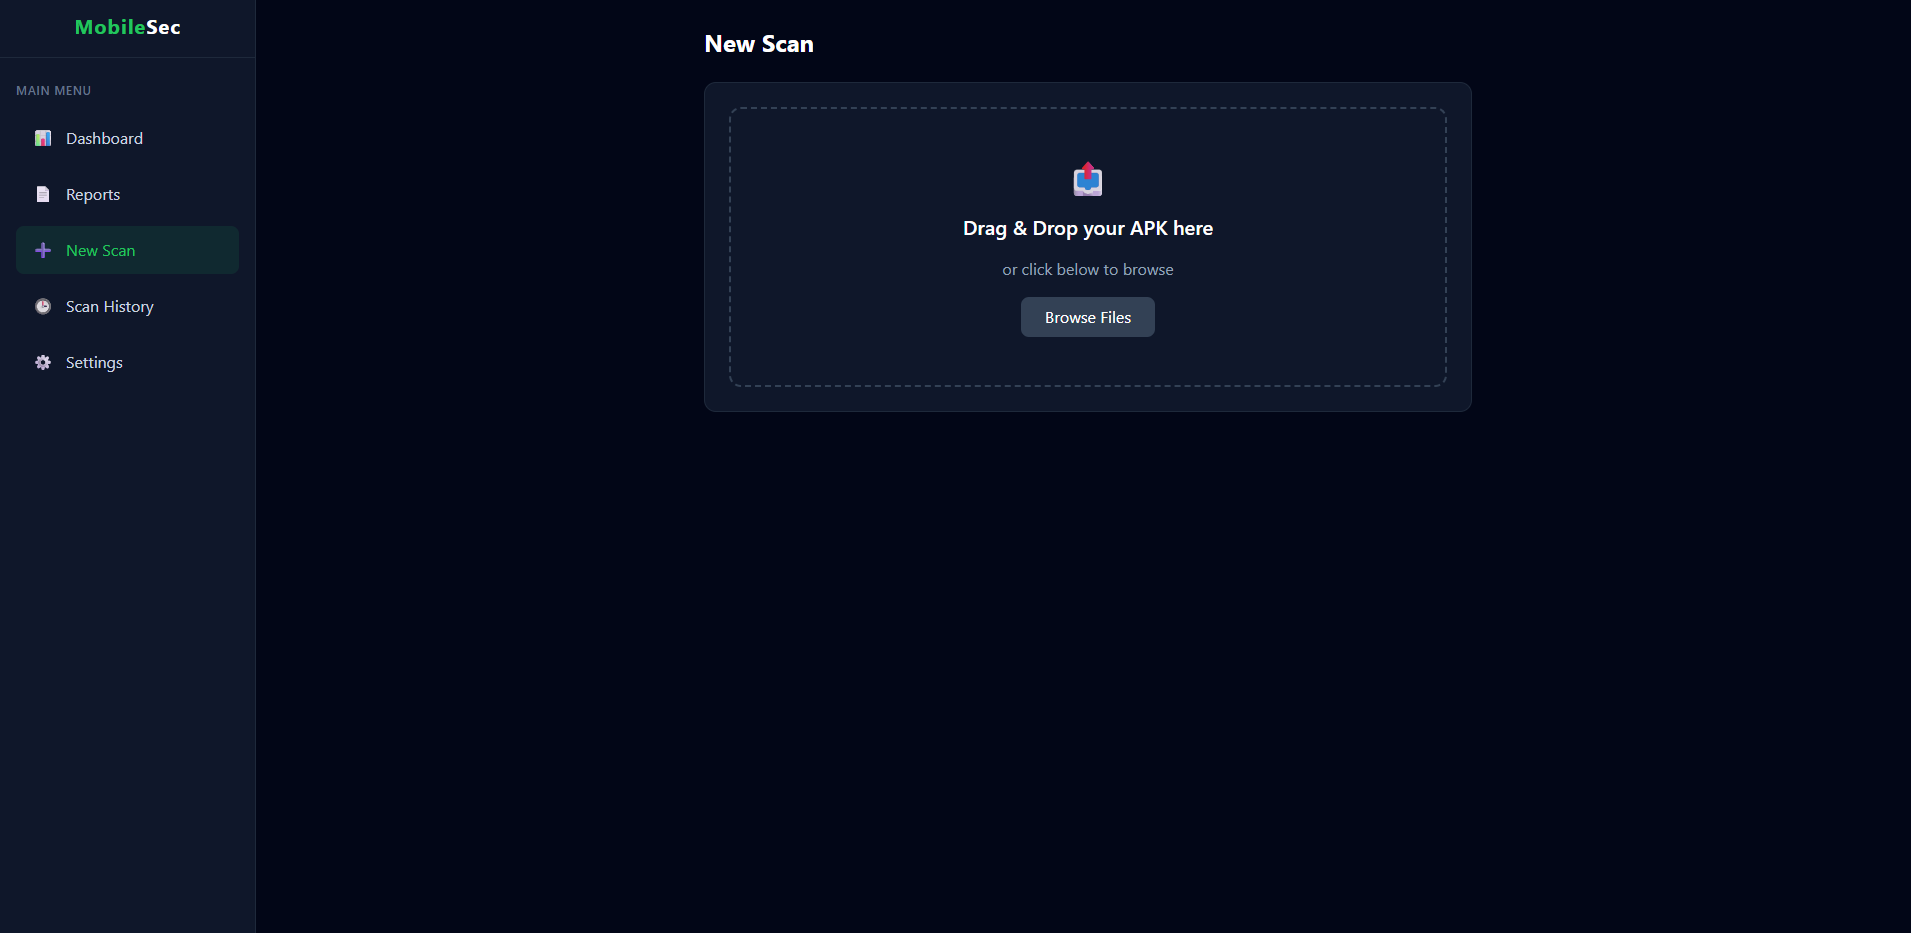
\includegraphics[width=\linewidth]{figures/dashboard.png}
    \caption{\textcolor{blue}{MobileSec dashboard summarizing detected vulnerabilities by category, severity level, and scan status after static APK analysis.}}
    \label{fig:dashboard}
\end{figure}

\subsection{Vulnerability prioritization and AI-assisted remediation}

%% humanized
After the static analysis is complete, MobileSec uses a LightGBM-based machine learning model to prioritize the detected vulnerabilities. The model assigns confidence scores and ranks the findings based on their estimated security impact. The frontend then displays a prioritized list of vulnerabilities, helping users quickly focus on the most critical issues. (Fig.~\ref{fig:prioritization}).

\begin{figure}[H]
    \centering
    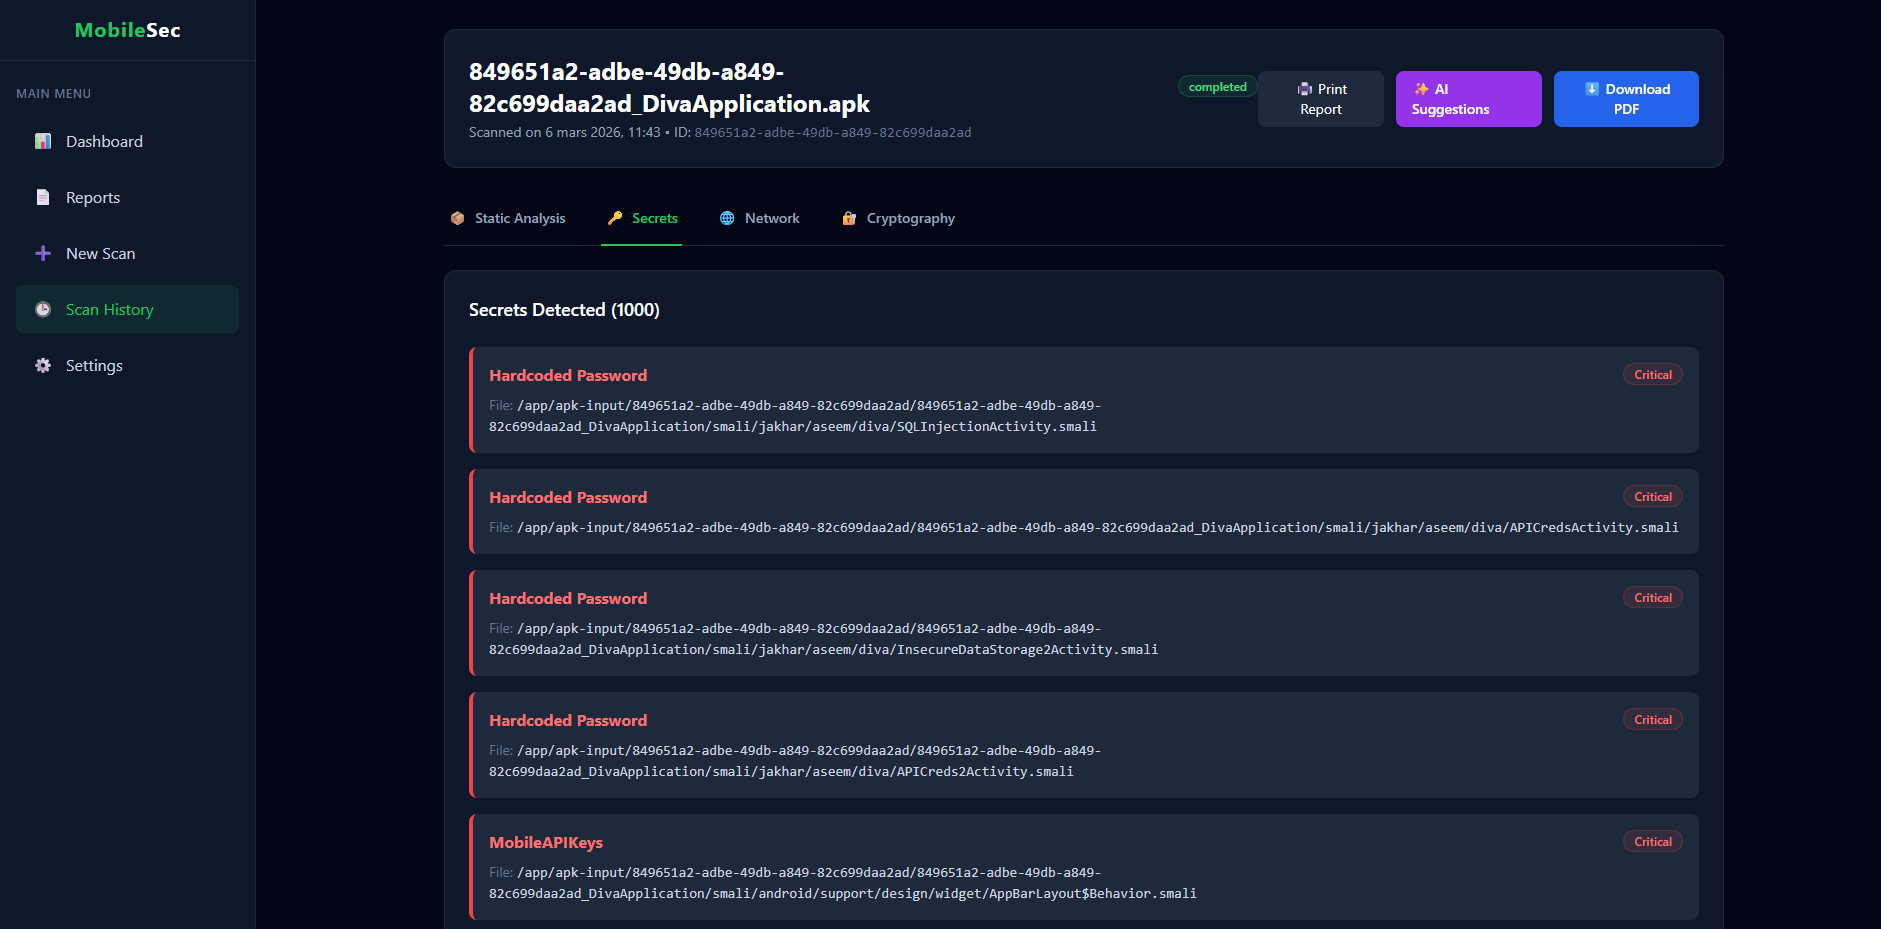
\includegraphics[width=\linewidth]{figures/prioritization.png}
    \caption{\textcolor{blue}{Prioritized vulnerability list ranked using the LightGBM-based machine learning model, highlighting critical findings.}}
    \label{fig:prioritization}
\end{figure}

%% humanized
For selected vulnerabilities, users can request AI-assisted remediation through the FixSuggest service. This component uses large language models accessed through the OpenRouter API to produce structured explanations of the security issue, step-by-step mitigation guidance, and complete Java or Kotlin code-level fix recommendations (Fig.~\ref{fig:fixsuggest}). The generated patches include the necessary imports and follow platform-specific development practices.

\begin{figure}[H]
    \centering
    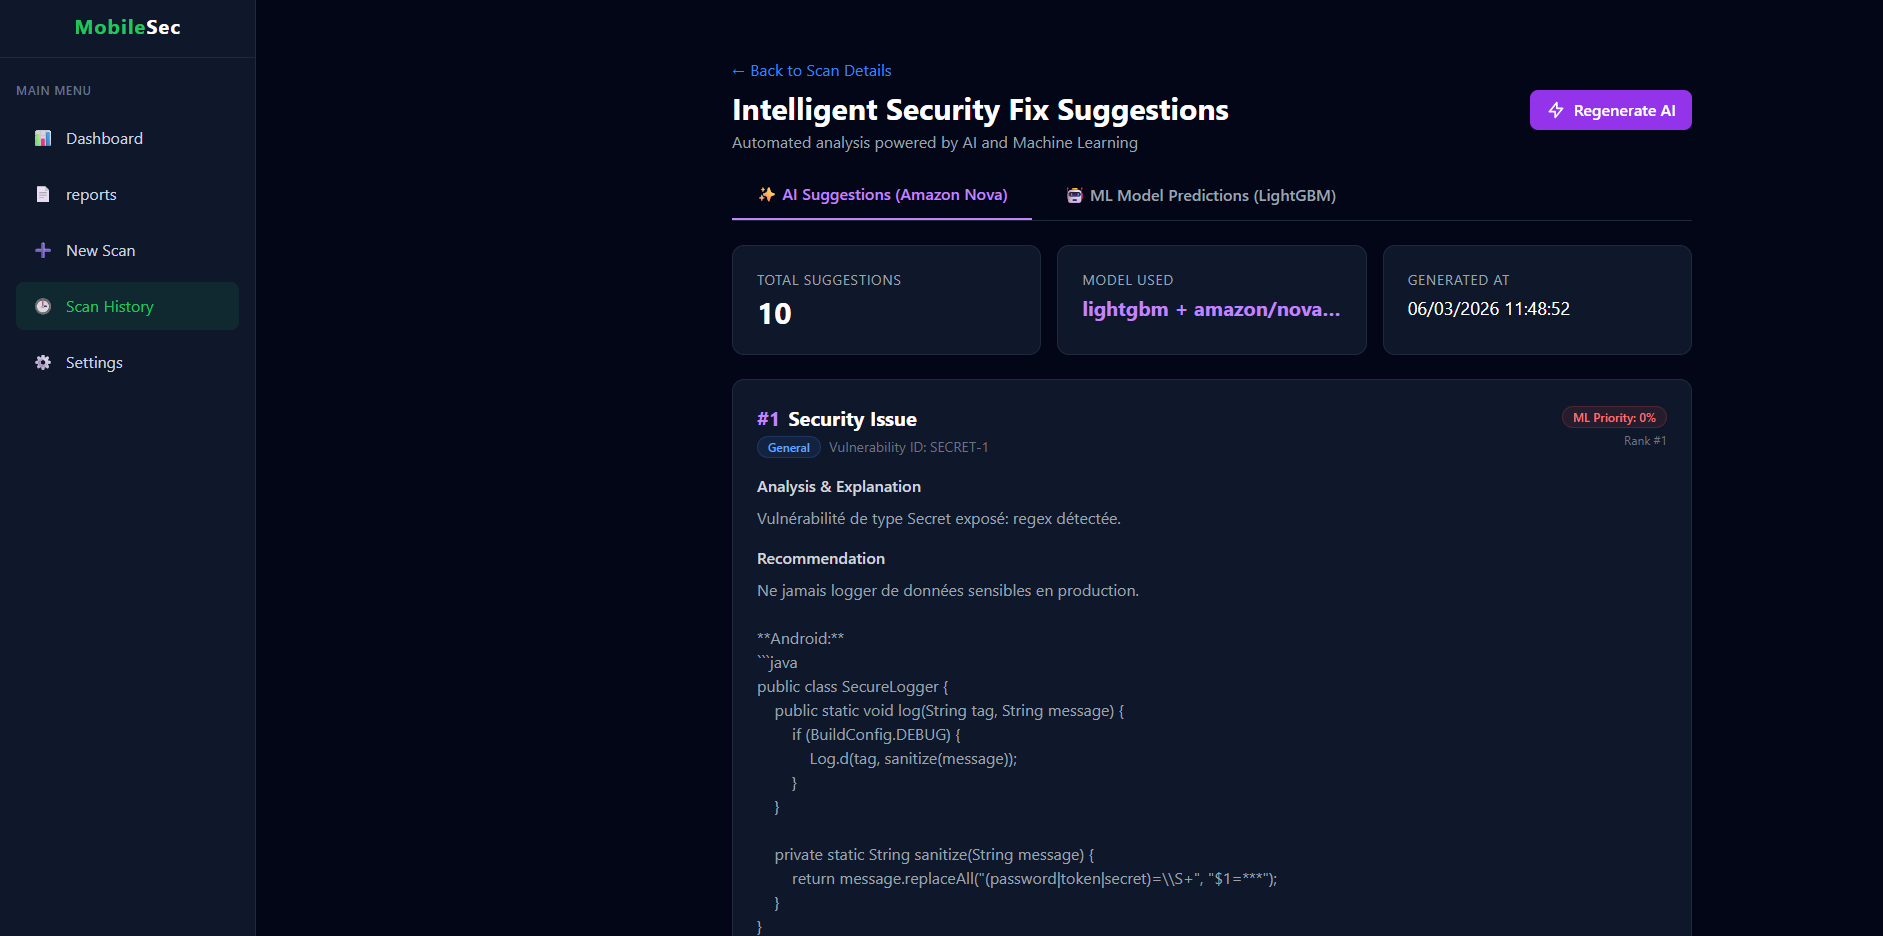
\includegraphics[width=\linewidth]{figures/fixsuggest.png}
    \caption{\textcolor{blue}{AI-assisted remediation interface showing vulnerability explanation and generated Java/Kotlin code-level fix suggestions.}}
    \label{fig:fixsuggest}
\end{figure}

%% humanized
The platform pairs machine learning–driven prioritization with AI-generated remediation guidance, helping developers concentrate on the most critical vulnerabilities while getting practical recommendations that reduce the need for manual analysis.

{\color{blue}\paragraph{Assessment scope of generated remediation.}
FixSuggest provides structured explanations and code-oriented remediation proposals through the implemented user workflow. The present evaluation demonstrates generation and presentation of these recommendations; it does not yet measure patch correctness, developer acceptance or time-to-remediate. These outcomes require a dedicated manual assessment protocol.}

\subsection{Automated security report generation}

%% humanized
MobileSec also makes it possible to automatically generate professional security reports. From the scan detail view, users can launch the ReportGen service to create a PDF report that summarizes all identified findings. The report contains an executive summary, a breakdown of vulnerabilities by category and severity, and detailed descriptions of each individual issue.

%% humanized
Generated reports are saved and can be accessed through a dedicated report history interface, where users are able to view, download, or delete earlier reports (Fig.~\ref{fig:report}). This feature helps teams communicate results to non-technical stakeholders and supports the use of MobileSec within formal security assessment and audit processes.

\textcolor{blue}{Report export was also verified during the benchmark experiment reported in Table~\ref{tab:mobilesec-benchmark-realworld-generated}: PDF, JSON and SARIF generation completed successfully for all 283 analyzed APKs.}

\paragraph{Explanation of how each penalty is calculated}
The generated report also presents an overall security score that summarizes the main risks identified during analysis. The score is calculated using a penalty-based approach in which the computation starts from 100 and subtracts weighted penalties for each detected issue category, including debuggable builds, cleartext traffic settings, risky permissions, insecure endpoints, hardcoded secrets, and exported components. To keep the score easy to read and compare across scans, the final value is clipped to the range \([0,100]\).

\begin{equation}
\begin{aligned}
\mathrm{Security\ Score} = \max \Bigl(
0,\,
100
&- \mathrm{debuggable\_penalty} \\
&- \mathrm{cleartext\_penalty} \\
&- \mathrm{permissions\_penalty} \\
&- \mathrm{insecure\_endpoints\_penalty} \\
&- \mathrm{hardcoded\_secrets\_penalty} \\
&- \mathrm{exported\_components\_penalty}
\Bigr)
\end{aligned}
\end{equation}

The different penalty terms are defined as follows:

\textbf{Debuggable penalty.} If the application is set to debug mode, a fixed deduction of 25 points is enforced:
    \[
    \mathrm{debuggable\_penalty}=
    \begin{cases}
    25 & \text{if the application is configured as debuggable} \\
    0 & \text{otherwise}
    \end{cases}
    \]

\textbf{Cleartext traffic penalty.} If unencrypted traffic is permitted, a fixed penalty of 15 points is imposed:
    \[
    \mathrm{cleartext\_penalty}=
    \begin{cases}
    15 & \text{if cleartext traffic is allowed} \\
    0 & \text{otherwise}
    \end{cases}
    \]

\textbf{Permissions penalty.} Let $R_{perm}$ represent the permission risk score calculated by the permissions analysis component. The corresponding deduction is:
    \[
    \mathrm{permissions\_penalty} = \min\left(\left\lfloor \frac{R_{perm}}{5} \right\rfloor, 20\right)
    \]
    Thus, every five permission risk points result in a one-point deduction, capped at a maximum penalty of 20.

\textbf{Insecure endpoints penalty.} Let $N_{endpoints}$ represent the number of insecure endpoints identified during the analysis. The penalty is calculated as:
    \[
    \mathrm{insecure\_endpoints\_penalty} = \min\left(2 \times N_{endpoints}, 15\right)
    \]
    Therefore, each insecure endpoint adds two penalty points, with the total penalty capped at 15.

\textbf{Hardcoded secrets penalty.} Let $N_{secrets}$ represent the number of hardcoded or potentially exposed secrets identified. The corresponding penalty is:
    \[
    \mathrm{hardcoded\_secrets\_penalty} = \min\left(3 \times N_{secrets}, 20\right)
    \]
    In this scenario, each detected secret adds three penalty points, with the total deduction capped at 20.

\textbf{Exported components penalty.} Let $N_{exported}$ represent the number of exported application components. No penalty is imposed when this value is five or less. Once it exceeds that threshold, the deduction is calculated as:
    \[
    \mathrm{exported\_components\_penalty} =
    \begin{cases}
    0 & \text{if } N_{exported} \leq 5 \\
    \min\left(N_{exported}-5, 10\right) & \text{if } N_{exported} > 5
    \end{cases}
    \]
    This indicates that each exported component beyond the initial five results in a one-point deduction, capped at a maximum of 10.

Once all penalties have been combined, the final score is bounded below at 0, meaning any negative value is set to 0. The implementation then assigns a qualitative grade based on the numeric score: \textit{A / Excellent} for scores of 80 or higher, \textit{B / Good} for scores between 60 and 79, \textit{C / Fair} for scores between 40 and 59, \textit{D / Poor} for scores between 20 and 39, and \textit{F / Critical} for scores below 20.

{\color{blue}\paragraph{Interpretation of the security score.}
The security score is designed as an interpretable triage indicator. Its penalties encode the relative attention assigned by the platform to detected issue types; they should not be interpreted as empirically calibrated probabilities of compromise or as a substitute for expert risk assessment. To examine the sensitivity of prioritisation to alternative weighting choices, the ranking produced by the implemented weights was compared with three alternative schemes.}

{\color{blue}
\begin{table}[H]
\centering
\caption{Sensitivity of security-score ranking to alternative weighting schemes.}
\label{tab:score-sensitivity}
\begin{tabular}{lrr}
\toprule
\textbf{Weighting scheme} & \textbf{Top-10 overlap} & \textbf{Kendall's $\tau$} \\
\midrule
Implemented weights & 1.00 & 1.0000 \\
Equal weights & 0.40 & 0.7658 \\
CVSS-inspired weights & 0.90 & 0.7765 \\
Secrets-emphasised weights & 0.90 & 0.6523 \\
\bottomrule
\end{tabular}
\end{table}
}

\textcolor{blue}{Formal calibration of the score against independently assessed application risk remains future work.}

\begin{figure}[H]
    \centering
    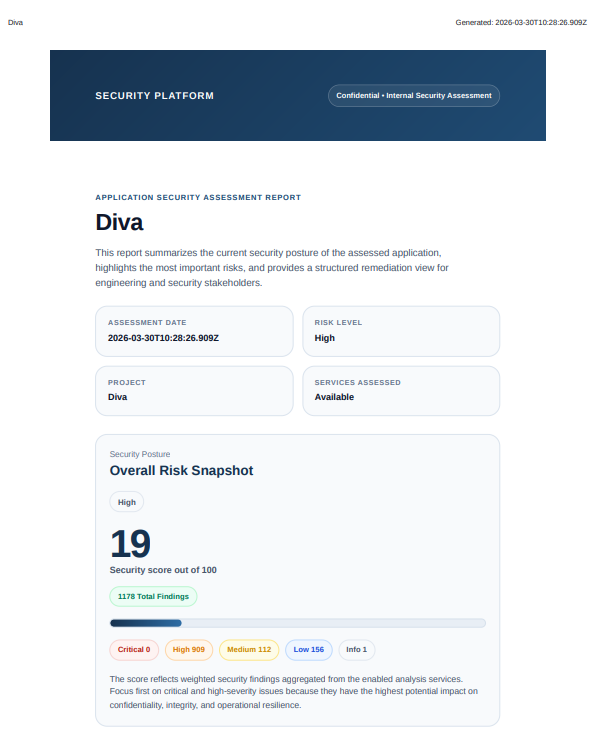
\includegraphics[width=\linewidth]{figures/report.png}
    \caption{\textcolor{blue}{MobileSec security report generation}}
    \label{fig:report}
\end{figure}

\section{Impact}

\textit{MobileSec} shifts Android security analysis from a fragmented sequence of separate tools toward a more unified and reproducible workflow. Rather than requiring analysts to move manually between decompilers, rule-based scanners, prioritization scripts, and reporting utilities, the platform brings these stages together within a single environment. This reduces practical overhead during experimentation and makes repeated analyses easier to reproduce. The platform also aligns with standardization efforts such as SARIF for the exchange of static-analysis results and with mobile-security guidance such as OWASP MASVS and MASTG, both of which emphasize structured and repeatable security assessment practices for mobile applications \cite{sarif2020,owaspmasvs,owaspmastg}.

From a research perspective, MobileSec provides a useful basis for studying how findings produced by different analyzers interact and how prioritization models behave under different configurations. Because outputs from multiple services are collected within the same pipeline, researchers can compare detector combinations, orchestration strategies, and ranking approaches without rebuilding the workflow for each experiment. This is especially relevant for benchmark-driven evaluation using resources such as DroidBench and Ghera \cite{arzt2014droidbench,ghera2017}.

\textcolor{blue}{The platform also improves day-to-day experimental practice. Intermediate artifacts, including manifest-derived information, certificate metadata, permissions and extracted endpoints, are stored for reuse, which reduces repeated preprocessing during iterative studies. The asynchronous orchestration mechanism decouples specialised analyzers; however, the benchmark reported here uses sequential APK processing because exploratory parallel executions did not consistently return complete analyzer outputs. The LightGBM prioritisation layer further moves the workflow beyond raw finding counts toward confidence-aware triage \cite{ke2017lightgbm}.}

\subsection{LightGBM prioritisation evaluation}

\textcolor{blue}{The prioritisation model is assessed on held-out labelled remediation outcomes. In addition to classification accuracy, macro-averaged measures are reported because they give equal weight to each remediation class. The area under the ROC curve (AUC) is reported using the multiclass one-versus-rest formulation. Table~\ref{tab:lightgbm-prioritization-generated} presents the persisted test results generated by the implemented evaluation workflow.}

{\color{blue}
\begin{table}[H]
\centering
\caption{Held-out performance of the LightGBM remediation-prioritisation model.}
\label{tab:lightgbm-prioritization-generated}
\begin{tabular}{lc}
\toprule
\textbf{Metric} & \textbf{Value} \\
\midrule
Accuracy & 0.6250 \\
Macro-precision & 0.7815 \\
Macro-recall & 0.6250 \\
Macro-F1 & 0.6284 \\
AUC & 0.9468 \\
False prioritisation rate & 0.3750 \\
Under-prioritisation rate & 0.1528 \\
Over-prioritisation rate & 0.1528 \\
\bottomrule
\end{tabular}
\end{table}

\begin{table*}[!htbp]
\centering
\caption{Comparison of remediation-prioritisation methods under the repeatable evaluation split.}
\label{tab:ml-baseline-comparison}
\begin{tabular}{lrrrrrr}
\toprule
\textbf{Model} & \textbf{Accuracy} & \textbf{Macro-precision} & \textbf{Macro-recall} & \textbf{Macro-F1} & \textbf{Top-3 acc.} & \textbf{AUC} \\
\midrule
Rule-based baseline & 0.2813 & 0.3128 & 0.2813 & 0.2473 & -- & -- \\
Logistic regression & 0.6667 & 0.8419 & 0.6667 & 0.6730 & 0.8854 & 0.9495 \\
Random forest & 0.6667 & 0.8485 & 0.6667 & 0.6635 & 0.8542 & 0.9498 \\
LightGBM & 0.6563 & 0.8239 & 0.6563 & 0.6532 & 0.8646 & 0.9484 \\
\bottomrule
\end{tabular}
\end{table*}

\begin{table*}[!htbp]
\centering
\caption{Examples of prioritisation errors observed in held-out predictions.}
\label{tab:lightgbm-errors}
\begin{tabular}{llllr}
\toprule
\textbf{Index} & \textbf{Expected category} & \textbf{Predicted category} & \textbf{Interpretation} & \textbf{Priority shift} \\
\midrule
0 & \texttt{FIX\_CRYPTO\_MEDIUM} & \texttt{FIX\_WEAK\_RSA\_KEY} & More specific cryptographic remediation predicted & +1 \\
3 & \texttt{FIX\_EXPOSED\_SECRET} & \texttt{FIX\_WEAK\_CIPHER} & Category error at the same priority level & 0 \\
4 & \texttt{FIX\_CRYPTO\_GENERAL} & \texttt{FIX\_WEAK\_RSA\_KEY} & More specific cryptographic remediation predicted & +1 \\
\bottomrule
\end{tabular}
\end{table*}
}

\textcolor{blue}{These results indicate that the model captures useful ordering information for remediation triage, while the observed errors show that predictions should remain reviewable rather than being treated as automated security decisions.}

For developers and security analysts, MobileSec supports an integrated scan-to-report workflow. Users can submit an APK, inspect prioritized findings, review remediation suggestions, and export structured reports without switching between disconnected tools. This reduces the time spent on normalizing outputs, reconciling severity levels, and preparing security documentation. Support for JSON and SARIF also makes the results easier to integrate into downstream platforms and audit processes \cite{sarif2020}.

Beyond academic use, MobileSec also has clear translational value for industrial settings. Its separation into scanning, detection, prioritization, remediation, and reporting services matches common deployment patterns in DevSecOps and enterprise software assurance, where gradual adoption and CI/CD integration are important practical considerations \cite{zhao2024devsecops,prates2025devsecops,mothanna2024security}. In this sense, the platform is not only a research prototype, but also a useful foundation for real-world software security workflows.

\subsection{Comparative analysis with MobSF, BeVigil, and Yaazhini}

To better situate \textit{MobileSec} within the broader mobile application security landscape, we compare it with three representative solutions: \textit{MobSF}, \textit{BeVigil}, and \textit{Yaazhini} (currently presented as the Vooki Android App Scanner). These tools were chosen because they reflect different usage models within the mobile security ecosystem: open-source automated analysis (\textit{MobSF}), large-scale application intelligence and risk discovery (\textit{BeVigil}), and Android/APK-focused vulnerability scanning with API-oriented capabilities (\textit{Yaazhini/Vooki}).

\textit{MobSF} is widely recognized as a comprehensive mobile security testing framework that supports both static and dynamic analysis, cross-platform application assessment, and exportable security reports. Based on its public documentation, it supports Android, iOS, and Windows applications, provides both static and dynamic testing features, and produces reports containing severity classifications, affected files, and remediation guidance. \textit{BeVigil}, in contrast, is positioned more as a mobile application security intelligence and search platform. Its public scanning interface highlights app risk scores, large-scale metadata search, code browsing, secret detection, and on-demand APK scanning. \textit{Yaazhini/Vooki AAS} primarily targets Android APK and API vulnerability analysis, reverse engineering, URL discovery, and detailed vulnerability reporting accompanied by risk ratings and mitigation-focused explanations.

Compared with these platforms, \textit{MobileSec} is designed as a microservices-based research and engineering platform focused on automated Android APK analysis. Its current implementation integrates APK preprocessing, specialized static analyzers for cryptographic misuse, secret exposure, and network-related weaknesses, a LightGBM-based prioritization module, AI-assisted remediation generation, PDF/JSON/SARIF-oriented reporting, and CI-oriented integration support. Rather than concentrating solely on vulnerability identification, \textit{MobileSec} explicitly links vulnerability detection with prioritization, explanation, remediation, and report generation in a unified end-to-end workflow.
{\small
\setlength{\tabcolsep}{4pt}
\renewcommand{\arraystretch}{1.2}

\begin{xltabular}{\textwidth}{%
>{\RaggedRight\arraybackslash}p{0.17\textwidth}
>{\RaggedRight\arraybackslash}X
>{\RaggedRight\arraybackslash}X
>{\RaggedRight\arraybackslash}X
>{\RaggedRight\arraybackslash}X}
\caption{\textbf{Qualitative comparison of MobileSec with representative mobile application security analysis platforms}} 
\label{tab:comparison_tools} \\
\toprule
\textbf{Criterion} & \textbf{MobileSec} & \textbf{MobSF\textsuperscript{1}} & \textbf{BeVigil\textsuperscript{2}} & \textbf{Yaazhini / Vooki AAS\textsuperscript{3}} \\
\midrule
\endfirsthead

\toprule
\textbf{Criterion} & \textbf{MobileSec} & \textbf{MobSF\textsuperscript{1}} & \textbf{BeVigil\textsuperscript{2}} & \textbf{Yaazhini / Vooki AAS\textsuperscript{3}} \\
\midrule
\endhead

\midrule
\multicolumn{5}{r}{\small Continued on next page} \\
\endfoot

\bottomrule
\endlastfoot

\textbf{Primary scope} 
& Android APK security analysis platform
& Mobile application security testing framework
& Mobile app security search and risk-intelligence platform
& Android APK and related API vulnerability scanner \\

\textbf{Architecture}
& Microservices-based
& Integrated framework
& Cloud/platform-oriented search and reporting workflow
& Scanner-oriented product workflow \\

\textbf{Platform emphasis}
& Android
& Android, iOS, Windows
& Mobile application ecosystem discovery and risk visibility
& Android APK and related APIs \\

\textbf{Static analysis}
& Yes
& Yes
& Partial / report-oriented exposure analysis
& Yes \\

\textbf{Dynamic analysis}
& Partial pipeline support through specialized services; mainly static in the current implementation
& Yes
& Not prominently documented as a dynamic runtime analysis framework
& API traffic capture / scanning workflow documented \\

\textbf{Cryptography checks}
& Yes
& Broad security checks
& Exposed through reported findings when detected
& Broad vulnerability scanning reported \\

\textbf{Secret detection}
& Yes
& Yes
& Yes, through extracted findings and exposed app data
& Broad vulnerability scanning reported \\

\textbf{Network analysis}
& Yes
& Yes
& Risk/report-oriented visibility over endpoints and app metadata
& Yes, especially through API scanning \\

\textbf{ML-based prioritization}
& Yes
& Not highlighted as a core documented feature
& Risk-score centric platform view
& Not highlighted as a core documented feature \\

\textbf{AI-assisted remediation}
& Yes
& Remediation guidance / documented findings
& Not highlighted as a core documented feature
& Mitigation / explanation support reported in product pages \\

\textbf{Report generation}
& PDF reports and structured outputs
& HTML / PDF / JSON export
& Security reports and risk score views
& Downloadable vulnerability reports \\

\textbf{CI / DevSecOps orientation}
& Yes
& Yes
& More search/intelligence oriented than CI-centric
& Not prominently emphasized in public documentation \\

\textbf{Research extensibility}
& High, due to modular microservices
& Moderate to high
& Lower for self-hosted experimental modification
& Moderate \\

\end{xltabular}
}
\vspace{0.3em}

\footnotetext[1]{\url{https://mobsf.github.io/Mobile-Security-Framework-MobSF/}}
\footnotetext[2]{\url{https://bevigil.com/}}
\footnotetext[3]{\url{https://www.vegabird.com/yaazhini/}}

The comparison shows that \textit{MobileSec} is not intended to simply mirror existing mobile scanning solutions. Rather, it establishes a distinct role by bringing together: (i) modular Android-focused security analysis, (ii) machine-learning-based vulnerability prioritization, (iii) AI-assisted remediation support, and (iv) integrated reporting and orchestration. These characteristics make it especially well suited for reproducible experimentation and for investigating how vulnerability detection, prioritization, and remediation assistance can be consolidated within a single platform.

\textcolor{blue}{The comparison in Table~\ref{tab:comparison_tools} is based on documented functional scope and deployment orientation. It situates MobileSec relative to established mobile-security platforms, but it does not by itself establish superior detection accuracy, execution time or remediation quality. Such claims require measurements obtained by executing each tool on the same APK set under comparable conditions.}

\subsection{Quantitative Comparison With Existing Tools}

\textcolor{blue}{The present experiment provides complete measured results for MobileSec on the DroidBench and Ghera benchmark suites. A numerical cross-tool table is not reported because comparable executions of MobSF, BeVigil and Yaazhini/Vooki on the identical 283-APK set are not yet available in the reproducibility artifacts. Once those measurements are obtained, the comparison will report runtime, detection outcomes, precision, recall, F1-score and report-export success using an identical evaluation protocol for each tool.}

\subsection{\textcolor{blue}{Benchmark evaluation on DroidBench and Ghera}}

\textcolor{blue}{The benchmark experiment was conducted on 283 APKs: 118 applications from DroidBench and 165 from Ghera. These suites provide reproducible test cases for evaluating detector behaviour and are reported separately because their composition and intended vulnerability scenarios differ. Archived MobileSec scan records without reference labels are not included in the accuracy calculation and are not used to support effectiveness claims.}

{\color{blue}
\begin{table*}[!htbp]
\centering
\caption{Measured MobileSec results on the complete DroidBench and Ghera APK sets.}
\label{tab:mobilesec-benchmark-realworld-generated}
\begin{tabular}{lrr}
\toprule
\textbf{Metric} & \textbf{DroidBench} & \textbf{Ghera} \\
\midrule
Number of APKs & 118 & 165 \\
Detected findings & 484 & 901 \\
True positives & 118 & 44 \\
False positives & 0 & 121 \\
False negatives & 0 & 0 \\
Precision & 1.0000 & 0.2667 \\
Recall & 1.0000 & 1.0000 \\
F1-score & 1.0000 & 0.4211 \\
Mean scan time & 4.29 s & 8.40 s \\
Mean CPU usage & 102.4\% & 70.5\% \\
Mean RAM usage & 276.8 MB & 555.2 MB \\
Throughput & 6.71 APK/min & 6.71 APK/min \\
Concurrent APK scans & 1 & 1 \\
Mean generated export size & 77165 bytes & 80304 bytes \\
Mean report-export time & 2.28 s & 2.24 s \\
PDF report success rate & 100.0\% & 100.0\% \\
SARIF export success rate & 100.0\% & 100.0\% \\
\bottomrule
\end{tabular}
\end{table*}
}

\textcolor{blue}{The results show complete recall on both suites, with substantially lower precision on Ghera due to false-positive detections in cases not expected to be reported as vulnerable. This distinction is important: the benchmark supports detection evaluation on its labelled cases, whereas operational scan archives require independent reference labelling before accuracy measures can be reported.}

\textcolor{blue}{Per-category precision and recall are not reported in this version because the benchmark annotation used for the current experiment does not yet contain a manually reviewed category assignment for each detected finding. This analysis is reserved for a subsequent annotation study.}

\textcolor{blue}{The current prioritisation evaluation has an additional scope limitation. MobileSec predicts an operational remediation category for an APK scan, while individual vulnerability ordering also incorporates severity-based signals. A future extension could train one instance per vulnerability and incorporate local evidence such as file location, detector source, CWE identifier, severity and surrounding code context.}

\subsection{\textcolor{blue}{Reproducibility and developer documentation}}

\textcolor{blue}{The benchmark workflow is reproducible from the repository services and evaluation scripts. The reported run analyzes the complete locally supplied DroidBench and Ghera APK collections and stores scan-detail, runtime-resource and benchmark-label outputs used to construct Table~\ref{tab:mobilesec-benchmark-realworld-generated}. The execution command is:}

{\color{blue}
\begin{verbatim}
node scripts/automate-paper-evaluation.js \
  --droidbench "<path-to-DroidBench-apks>" \
  --ghera "<path-to-Ghera-apks>" \
  --api "http://localhost:5000" \
  --reportgen "http://localhost:3005" \
  --concurrency 1 --derive-ground-truth
\end{verbatim}
}

\textcolor{blue}{DroidBench and Ghera remain third-party benchmark resources and must be obtained and used according to their corresponding distribution conditions. The repository documentation describes the service configuration, principal endpoints and the procedure for extending the platform with additional analysis services.}

\section{Conclusions}

%% humanized
This work introduced \textit{MobileSec}, a modular platform for Android security assessment that brings together static APK analysis, specialized vulnerability detection, machine learning–based prioritization, AI-assisted remediation, and multi-format reporting within a single workflow. In doing so, the platform addresses a practical limitation in current mobile security practice: while many tools are able to identify issues, far fewer offer a complete path from raw findings to prioritized and actionable remediation.

%% humanized
\textcolor{blue}{From an engineering standpoint, MobileSec demonstrates that a microservices-based architecture can organize heterogeneous Android security analyses while preserving reproducible deployment through containerisation. The current implementation includes domain-specific components for cryptography, secret exposure and network-related risk, coordinated through persistent scan-state management and asynchronous messaging. Its operational costs and current concurrency limitation are explicitly reported in this article.}

%% humanized
One of the main contributions of the platform is its combination of deterministic analysis results with data-driven triage and remediation support. The LightGBM-based prioritization service converts findings from multiple sources into ranked recommendations accompanied by confidence estimates, while the FixSuggest component enhances findings with MASVS-aligned and LLM-assisted remediation guidance. Together, these capabilities help reduce analyst burden and make static analysis results more practical and usable.

%% not humanized
\textcolor{blue}{The LightGBM evaluation shows that scan-level features can support remediation-oriented triage, while the benchmark experiment provides measured detection and reporting results for DroidBench and Ghera. Archived scans without reference labels are treated as descriptive platform records and are not included in accuracy claims.}

%% humanized
MobileSec also improves communication and integration. Support for PDF, JSON, and SARIF report generation enables both human-readable and machine-consumable outputs, while CI-oriented endpoints make it easier to integrate the platform into DevSecOps pipelines. These features broaden the software’s usefulness across research environments, educational contexts, and industrial security operations.

{\color{blue}\paragraph{Limitations.}
The present evaluation has four principal limitations. First, detection metrics are reported for DroidBench and Ghera benchmark APKs and should not be generalized to archived or production applications without independent reference labelling. Second, numerical comparison with MobSF, BeVigil and Yaazhini/Vooki requires equivalent executions on the same APK set and is not claimed in this article. Third, the security-score weighting scheme and FixSuggest recommendations require further expert and user-centred assessment. Finally, the reported benchmark uses sequential APK execution, because exploratory parallel executions did not provide consistently complete analyzer outputs.}

%% humanized
Future work will concentrate on large-scale empirical benchmarking, stronger evaluation datasets, expanded detector coverage, and more rigorous assessment of remediation effectiveness, including metrics such as fix acceptance rate, time to remediate, and false-positive impact. Other directions include stronger policy enforcement for enterprise deployments, better explainability for ranking decisions, and continuous retraining of models using historical scan feedback. Overall, MobileSec offers a strong and extensible foundation for reproducible Android security analysis and practical vulnerability management.

\begin{thebibliography}{00}

\bibitem{arzt2014flowdroid}
S.~Arzt, S.~Rasthofer, C.~Fritz, E.~Bodden, A.~Bartel, J.~Klein, Y.~Le~Traon,
D.~Octeau, and P.~McDaniel,
FlowDroid: Precise context, flow, field, object-sensitive and lifecycle-aware taint analysis for Android apps,
\textit{ACM SIGPLAN Notices}, vol.~49, no.~6, pp.~259--269, 2014.

\bibitem{enck2014taintdroid}
W.~Enck, P.~Gilbert, B.-G.~Chun, L.~P.~Cox, J.~Jung, P.~McDaniel, and A.~Sheth,
TaintDroid: An information-flow tracking system for realtime privacy monitoring on smartphones,
\textit{ACM Transactions on Computer Systems}, vol.~32, no.~2, 2014.

\bibitem{feng2014apposcopy}
Y.~Feng, S.~Anand, I.~Dillig, and A.~Aiken,
Apposcopy: Semantics-based detection of Android malware through static analysis,
in \textit{Proceedings of the ACM SIGSOFT International Symposium on the Foundations of Software Engineering (FSE)}, 2014.

\bibitem{li2017iccta}
L.~Li, A.~Bartel, T.~F.~Bissyand\'e, J.~Klein, Y.~Le~Traon, and S.~Arzt,
IccTA: Detecting inter-component privacy leaks in Android apps,
in \textit{Proceedings of the IEEE/ACM International Conference on Automated Software Engineering (ASE)}, 2017.

\bibitem{desnos2011androguard}
A.~Desnos,
Androguard: Reverse engineering, malware and goodware analysis of Android applications,
in \textit{Black Hat Europe}, 2011.

\bibitem{arzt2014droidbench}
S.~Arzt, J.~Klein, and E.~Bodden,
DroidBench: A benchmark for Android taint analysis,
in \textit{Proceedings of the International Conference on Software Engineering Companion (ICSE-C)}, 2014.

\bibitem{liu2021mlsecurity}
Y.~Liu, Y.~Wang, and J.~Sun,
Machine learning for software vulnerability detection: A systematic review,
\textit{IEEE Transactions on Reliability}, vol.~70, no.~3, pp.~1187--1214, 2021.

\bibitem{ke2017lightgbm}
G.~Ke, Q.~Meng, T.~Finley, T.~Wang, W.~Chen, W.~Ma, Q.~Ye, and T.-Y.~Liu,
LightGBM: A highly efficient gradient boosting decision tree,
in \textit{Advances in Neural Information Processing Systems (NeurIPS)}, 2017.

\bibitem{pearce2022copilot}
H.~Pearce, B.~Ahmad, B.~Tan, B.~Dolby, and S.~Elbaum,
Asleep at the keyboard? Assessing the security of GitHub Copilot’s code contributions,
in \textit{Proceedings of the IEEE Symposium on Security and Privacy}, 2022.

\bibitem{white2023prompt}
J.~White, S.~Hays, Q.~Fu, J.~Spencer-Smith, and D.~C.~Schmidt,
A prompt pattern catalog to enhance prompt engineering with ChatGPT,
\textit{arXiv preprint arXiv:2302.11382}, 2023.

\bibitem{owaspmasvs}
OWASP Foundation,
OWASP Mobile Application Security Verification Standard (MASVS),
Available online: \url{https://mas.owasp.org/MASVS/},
accessed 2026.

\bibitem{sarif2020}
OASIS,
Static Analysis Results Interchange Format (SARIF) Version 2.1.0,
OASIS Standard, 27 March 2020.
Available online: \url{https://docs.oasis-open.org/sarif/sarif/v2.1.0/sarif-v2.1.0.html}.

\bibitem{owaspmastg}
OWASP Foundation,
OWASP Mobile Application Security Testing Guide (MASTG),
Available online: \url{https://mas.owasp.org/MASTG/},
accessed 2026.

\bibitem{ghera2017}
V.~P.~Ranganath and S.~Mitra,
Ghera: A Repository of Android App Vulnerability Benchmarks,
in \textit{Proceedings of the 14th International Conference on Mining Software Repositories (MSR)}, 2017.

\bibitem{zhao2024devsecops}
X.~Zhao, et al.,
Identifying the primary dimensions of DevSecOps: A multivocal literature review and thematic analysis,
\textit{Journal of Systems and Software}, vol.~218, 2024.

\bibitem{prates2025devsecops}
L.~Prates, et al.,
DevSecOps practices and tools,
\textit{International Journal of Information Security}, 2025.

\bibitem{mothanna2024security}
Y.~Mothanna, et al.,
Adopting security practices in software development process,
\textit{Computers \& Security}, vol.~147, 2024.

\end{thebibliography}

\end{document}
\endinput
%%
%% End of file `SoftwareX_article_template.tex'.

%%% Local Variables:
%%% mode: latex
%%% TeX-master: t
%%% End:
